\documentclass{article}
\usepackage{amsthm}
\usepackage{amsmath}

%%%%%%%%%%%%%%%% Tikz and pgf %%%%%%%%%%%%%%%%%%%%%5
\usepackage{tikz}
%\usepackage{pgfmath}
\usetikzlibrary{positioning, arrows,automata}
\usetikzlibrary{shapes}

%%%%%%%%%%%%%%%%%%%%%%%%%%%%%%%%%%%%%%%%%%%%%%%%%%%%%

\usepackage{dot2texi}



\newtheorem{theorem}{Theorem}[section]
\title{How to make money using Number theory?}
\author{Dofus M Bofus}
\begin{document}
\maketitle

\section{Introduction}

For a complex number $s$, we consider the series.

\begin{equation}
  \zeta(s) = \sum_{n=1}^\infty \frac{1}{n^s}
  \label{eq-riemann-zeta}
\end{equation}

\begin{theorem}
  Consider the analytic continuation of the \emph{Riemann zeta function}
  defined in Equation~\ref{eq-riemann-zeta}. All the non-trivial roots
  of it lie on the $\mathrm{Re}(s)=\frac{1}{2}$ line.
\end{theorem}

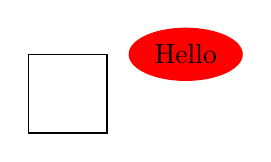
\begin{tikzpicture}
  \draw[-] (0,0) -- (0,1) -- (1,1) -- (1,0) -- (0,0);
  \node[fill=red, shape=ellipse] at (2,1) {Hello};
\end{tikzpicture}

\section{An NFA}

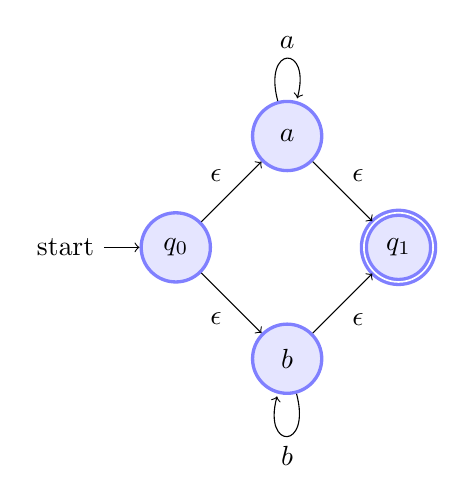
\begin{tikzpicture}[node distance=2cm, auto]
  \tikzstyle{every state}=[shape=circle, draw=blue!50, very thick, fill=blue!10];
  \node [state, initial] (q) at (0,0)         (q0)   {$q_0$};
  \node [state, above right of= q0]           (a)    {$a$};
  \node [state, below right of= q0]           (b)    {$b$};
  \node [state, above right of= b, accepting] (q1)   {$q_1$};

  \path[->] (q0) edge node[above left]{$\epsilon$} (a)
                 edge node[below left]{$\epsilon$} (b);

  \path[<-] (q1) edge node[above right]{$\epsilon$} (a)
                 edge node[below right]{$\epsilon$} (b);

  \path[->] (a) edge [loop above] node {$a$} ();
  \path[->] (b) edge [loop below] node {$b$} ();


\end{tikzpicture}


\section{Drawing graphs}


\begin{dot2tex}[neato,mathmode]
  digraph G {
    node[shape=circle];
    a_1 -> a_2 -> a_3 -> a_4 -> a_5 -> a_1;
  }
\end{dot2tex}


\section{Automata using graphviz and tikz}

\begin{tikzpicture}
  \tikzstyle{every state}=[shape=circle, draw=blue!50, very thick, fill=blue!10];
  \begin{dot2tex}[styleonly,codeonly,circo, mathmode]
    
    digraph G {
      d2ttikzedgelabels = true;
      node[style="state"];
      edge[lblstyle="auto", topath="bend left"];

      A -> A
      A -> B
      B -> C
      C -> C
      C -> A
    }
  \end{dot2tex}
\end{tikzpicture}


\section{Plotting graphs}

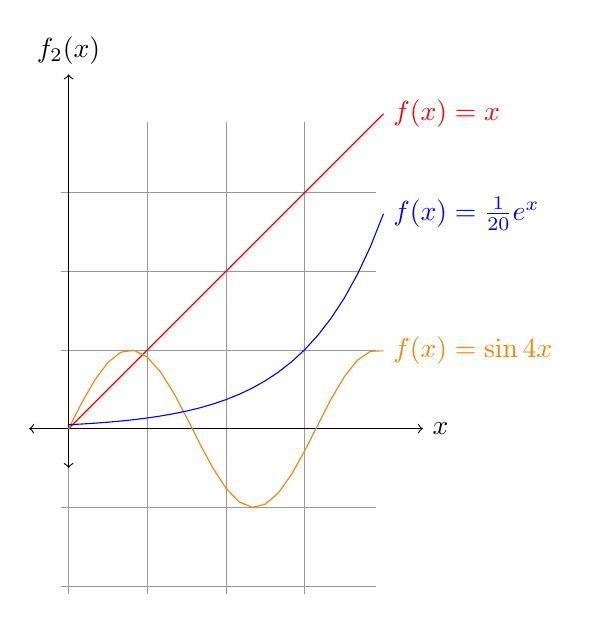
\begin{tikzpicture}[domain=0:4]
  \draw[very thin, color=black!40] (-0.1,-2.1) grid (3.9,3.9);
  \draw[<->] (-0.5,0) -- (4.5,0) node [right] {$x$};
  \draw[<->] (0,-0.5) -- (0,4.5)  node [above] {$f_2(x)$};
  \draw[color=red] plot (\x,\x) node [right] {$f(x) = x$};
  \draw[color=orange] plot (\x,{sin(2*\x r)}) node [right] {$f(x) = \sin {4}x$};
  \draw[color=blue] plot (\x,{0.05*exp(\x)}) node [right] {$f(x) = \frac{1}{20}e^x$};
\end{tikzpicture}


\end{document}
